\documentclass{article}

\usepackage[english]{babel}
\usepackage{amsmath}
\usepackage{amssymb}
\usepackage{amsthm}
\usepackage[letterpaper,top=2cm,bottom=2cm,left=3cm,right=3cm,marginparwidth=1.75cm]{geometry}
\usepackage{graphicx}
\usepackage[colorlinks=true, allcolors=blue]{hyperref}
\usepackage{fancyhdr}
\usepackage{tikz}
\usetikzlibrary{decorations.markings,calc}
\usepackage{tikz-cd}
\usepackage{quiver}
\usetikzlibrary{matrix}
\usepackage[most]{tcolorbox}
\usepackage{hyperref}
\usepackage{array}
\usepackage{colonequals}
\usepackage{todonotes}
\usepackage{theoremref}

\font\maljapanese=dmjhira at 2.5ex
\newcommand{\yo}{\textrm{\!\maljapanese\char"48}}

\newtheorem{theorem}{Theorem}[section]

\theoremstyle{definition}
\newtheorem{definition2}[theorem]{Definition}
\newtheorem{lemma}[theorem]{Lemma}
\newtheorem{corollary}[theorem]{Corollary}
\newtheorem{definition}[theorem]{Definition}
\newtheorem{example}[theorem]{Example}
\newtheorem{examples}[theorem]{Examples}


\theoremstyle{remark}
\newtheorem*{remark}{Remark}

\theoremstyle{plain}
\newtheorem{proposition}[theorem]{Proposition}
\newtheorem{conjecture}[theorem]{Conjecture}


\newcommand{\R}{\mathbb{R}}
\newcommand{\C}{\mathbb{C}}
\newcommand{\Z}{\mathbb{Z}}
\newcommand{\N}{\mathbb{N}}
\newcommand{\Q}{\mathbb{Q}}
\newcommand{\mb}[1]{\mathbb{#1}}
\newcommand{\mc}[1]{\mathcal{#1}}
\newcommand{\mk}[1]{\mathfrak{#1}}
\newcommand{\un}{\cup}
\newcommand{\ic}{\cap}
\pagestyle{fancy}
\newcommand\size{1}% distance of nodes from center

\usepackage{microtype}

\usepackage{caption}
\captionsetup[figure]{labelformat=empty}%

\begin{document}


\title{The \'Etale Fundamental Group}
\author{Daniel Ao}

\maketitle

\tableofcontents

\section{Introduction}

The fundamental group is an important invariant that appears in algebraic topology and it is a natural question to ask if there is an analog in the algebro-geometric setting.
Every scheme has an associated topological space, so one may naively apply the definitions from algebraic topology; however, the topology on schemes is generally too coarse for us to obtain anything of value.
A more fruitful approach instead uses the fundamental group's relation to theory of covers, of which there is a satisfactory schematic analog in finite \'etale covers which we lay out in Section 3.\\

What may not be immediately obvious is that the \'etale fundamental group is intimately related to that of Galois theory for field extensions. 
In fact, as an easy corollary at the end of Section 3 we will prove \thref{grothendiecksformulation}, a (albeit slightly different) formulation of Krull's theorem for Galois extensions.
Before, this however, we will establish some necessary foundation in Galois Theory and the topological fundamental group. 
And although we may initially have cautioned against a relation between the topological and \'etale fundamental group, there are still contexts where one can say a lot about the other.
Near the end, we will look at one possibility in \thref{RiemannExistence}, which relates the two in the case of finite type schemes over $\C$ and see some immediate uses.\\

\indent We will roughly follow \cite{Szamuely}, in particular during our construction of the \'etale fundamental group we will try and emphasize the similarity to the topological case.
One may find many similar notions between Galois theory and both the \'etale and topological cases which we will point out.
These are adequately addressed in a more axiomatic treatment involving Galois categories, for which one may look at Grothendieck's original work (\cite{grothendieck}) or at \cite{Lenstra}.

\section{Preliminaries}
We will first go over some important concepts that we will be necessary in our development.
Here we go over the important notion of a profinite group, and extend our knowledge of Galois theory for finite extensions to the possibly infinite case.

\subsection{Infinite Galois Theory}

Following the notation of \cite{Szamuely} we will denote a field extension $K \supseteq k$ as $K|k$. 
Now as we know, for finite Galois extensions $K|k$ there is an inclusion-reversing bijection between subfields $K \supseteq L \supseteq k$ and subgroups $H \subset \text{Gal}(K|k)$.
In particular, a subfield $L$ is assigned the subgroup $\text{Aut}(K|L) \subset \text{Gal}(K|k)$ fixing $L$ and a subgroup $H$ is assigned its fixed field $K^H$.
Unfortunately, for infinite Galois extensions this correspondence breaks down.
However, there is still a satisfactory correspondence which we will look at.\\

For preliminaries, first note that any partially ordered set $(\Lambda, \leq)$ can be viewed as a category where the objects are elements of $\Lambda$, and there is a morphism between $a,b \in \Lambda$ if and only if $a \leq b$.
Call a partially ordered set $(\Lambda, \leq)$ \textit{directed} if for all $c_1, c_2 \in \Lambda$ there exists a $d \in \Lambda$ such that $c_1 \leq d, c_2 \leq d$.

\begin{definition}
	Let $\mc{C}$ be a category and $J$ a directed partially ordered set. A \textit{(filtered) inverse system} of $\mc{C}$ is a contravariant functor $F: J^{\text{op}} \to \mc{C}$.
\end{definition}

If the limit of an inverse system $F: J^{\text{op}} \to \mc{C}$ exists, we will call it an \textit{inverse limit}.
It will be denoted as $\varprojlim C_{j}$, where $\{C_j\}_{j \in J}$ are the objects in $\mc{C}$ indexed by $J$.
When $\mc{C}$ is the category of groups, the limit always exists and it is the subgroup of $\prod_{j \in J} G_j$ consisting of sequences $(g_i)$ such that $Fk(g_i) = g_j$ if there is a morphism $k: i  \to j$ in $\Lambda$.

\begin{definition}
	A profinite group is the inverse limit of an inverse system whose objects are all finite groups.
\end{definition}

\begin{remark}
	There is a fundamental topology on any profinite group which we will make use of in the statement of Krull's theorem.
	In particular, if $G$ is a profinite group which is the inverse system of finite groups $\{G_i\}_{i \in I}$ we may give each $G_j$ the discrete topology.
	These define a product topology on $\prod_{i \in I} G_i$, and so $G$ viewed as a subgroup can be equipped with the natural subspace topology.
	We give some facts about this topology below.
\end{remark}
	
\begin{proposition}
	Let $G = \varprojlim G_i$ be a profinite group and consider the topology mentioned above.
	The following hold:
	\begin{enumerate}
		\item $G$ is a closed subgroup of $\prod G_i$.
		\item $G$ is compact and totally disconnected.
		\item Open subgroups of $G$ are precisely closed subgroups of finite index.
	\end{enumerate}
	
	\begin{proof}
		We first show that $G$ is closed in $\prod G_i$.
		Let $G$ be the inverse limit of groups $\{G_i\}_{i \in I}$ with maps $\phi_{\alpha \beta}: G_{\beta} \to G_{\alpha}$. 
		If $x \notin G$, then it is a sequence $(g_i)_{i \in I} \subset \prod G_i$ such that $\phi_{\alpha \beta} (g_{\beta}) \neq g_{\alpha}$for some finite groups $G_{\alpha}$ and $G_{\beta}$.
Then consider the following subset of $\prod G_i$
\[S  = \{(h_i) \,|\, h_{\beta} = g_{\beta}, h_{\alpha} \neq g_{\alpha}\}\]
If $\pi_{\alpha}$ and $\pi_{\beta}$ are the natural projections of $\prod G_i$ onto $G_{\alpha}$ and $G_{\beta}$, $S$ is the intersection of $\pi_{\alpha}^{-1}(G_{\alpha} - g_{\alpha})$ and $\pi_{\beta}^{-1}(g_{\beta})$, which are open by continuity of the projection maps and the discrete topology on each $G_i$.
Hence $S$ is an open subset containing $x$ but not intersecting $G$, hence $G$ is closed.\\
\indent For the second statement, since each $G_i$ is finite, it is compact with the discrete topology.
By Tychonoff's theorem $\prod G_i$ is also compact, hence $G$ is compact being a closed subset of a compact space.
To show that $G$ is totally disconnected, consider any two distinct points $(f_i)_{i \in I}, (g_i)_{i \in I} \in \prod G_i$.
Then $f_{\alpha} \neq g_{\alpha}$ for some $\alpha \in I$.
Using the same notation as in the first part of the proof, $\pi_{\alpha}^{-1}(f_{\alpha})$ and $\pi_{\alpha}^{-1}(G_{\alpha} - f_{\alpha})$ are both open and closed by the discrete topology on $G_{\alpha}$, which separate both $(f_i)_{i \in I}$ and $(g_i)_{i \in I}$.
Therefore any subset with more than 2 elements cannot be disconnected, hence the only connected subsets must trivially be the singeletons, hence $G$ is totally disconnected.\\
\indent Finally, we prove the third statement.
Since the maps $U \to gU$ are continuous for any topological group, each left coset $gU$ is open in $G$.
Since they partition $G$, $U$ must also be closed as its complement is a union of its open left cosets.
Since $G$ is compact there must only be finitely many such cosets.
Conversely, by similar reasoning a closed group of finite index has its complement a finite union of closed cosets, and so is open.
\end{proof}
	
\end{proposition}

\begin{examples} \text{}
\begin{enumerate}
	\item For any group $G$, the set of finite quotients is naturally an inverse system.
		In particular, there is a partial order on the set of normal subgroups of finite index where we let $H_1 \leq H_2$ if $H_1 \supseteq H_2$, and corresponding quotient maps between the associated groups $G/H_1 \to G/H_2$.
		The inverse limit of this system is called the \textit{profinite completion} of $G$ which we will denote as $\widehat{G}$.	
		The natural projection maps $G \to G/H_i$ commute with the system, and hence define a canonical map $G \to \widehat{G}$ from the property of limits.
	\item The Galois group for any field extension $K|k$ is a profinite group, as we will prove below.
		\end{enumerate}
\end{examples}


\begin{proposition}
	If $K|k$ is a Galois field extension then $\text{Gal}(K|k)$ is a profinite group.
	In particular, it is the inverse limit of an inverse system consisting of the groups $\text{Gal}(L|k)$ for finite Galois subextensions $K \supset L \supset k$.
\end{proposition}
\begin{proof}
	The inverse system consists of the Galois groups $\text{Gal}(L|k)$ for $L$ finite Galois subextensions of $K|k$.
	There are homomorphisms $\phi_{L_1L_2}: \text{Gal}(L_1|k) \to \text{Gal}(L_2|k)$ for subextensions whenever $L_1 \supset L_2 \supset k$ obtained by restricting the $k$ automorphisms of $L_2$ to $L_1$; this system is directed as the compositum $L_1 L_2$ of Galois extensions is also Galois.\\
\indent We construct the isomorphisms as follows.
There is a map $\phi: \text{Gal}(K|k) \to \prod \text{Gal}(L|k)$ over all finite Galois extensions $L|k$, which for any $k$-automorphism $\sigma$ of $\text{Gal}(K|k)$ sends it to the direct product of its restrictions to each extension $L$.
Since each $L$ is Galois, we have that the restriction of $\sigma$ to $L$ is also an automorphism of $L$ hence $\phi$ is well-defined.
Now first note that $\phi$ is injective, as if an automorphism $\sigma$ of $K|k$ does not fix an element $x$ of $K$, then it does not fix some finite Galois subextenion containing $x$ (for example the splitting field of its minimal polynomial).
Now the image of $\phi$ must lie in $\varprojlim \text{Gal}(L|k)$ as  $\sigma_{L_2} = \phi_{L_1 L_2} \sigma_{L_1}$ as both simply restrict $\sigma$ to $L_2$.
Finally, we show that the map is surjective.
For any $(\sigma_L) \in \varprojlim \text{Gal}(L|k)$ we can form a $k$-automorphism  $\sigma$ of $k$ by letting $\sigma(x) = \sigma_L(x)$ for a finite Galois subextension $L$ containing $x$. 
This is well-defined as $(\sigma_L)$ is by assumption a compatible system, and hence there is a $\sigma$ such that $\phi(\sigma) = (\sigma_L)$ as we want to show.
\end{proof}

\begin{example}
	Let $\mathbb{F}_p$ be a field of characteristic $p$.
	Denote 
\todo{Could be nontrivial example}

\end{example}
We may give the statement of Krull's theorem, which covers the case of infinite Galois extensions.
The bijection from the finite case fails as not all subgroups arise as one fixing a subextension, but thankfully the set of such subgroups has a nice description using the topology on the Galois group.
\begin{theorem}[Krull]\thlabel{Krull}
	Let $K | k$ be a Galois extension.
	If $k \subseteq L \subseteq K$ is a subestension, then $\text{Gal}(K|L)$ is a closed subgroup of $\text{Gal}(K|k)$.
	In particular, for subextensions $L$ and closed subgroups $H \subset \text{Gal}(K|k)$ the maps $H \to K^H$ and $L \to \text{Gal}(K|L)$ form an inclusion reversing bijection.
\end{theorem}

\begin{proof}
	For a proof see \cite{Szamuely}, Theorem 1.3.11. 
\end{proof}


\begin{remark}
	One may note just from the statement of the above theorem that this will only differs from the case with finite extensions if there exist nonclosed subgroups for some Galois group.
	The first one to construct such an example is \todo{cite Krull and finish}, which in fact 
\end{remark}

We will rephrase \thref{Krull} in a more useful form by putting it in a categorical context, the next notion will be important in this regard, as well as in the construction of the \'etale fundamental group.

\begin{definition} \thlabel{etalealgebra}
	A finite-dimensional $k$-algebra $A$ is \textit{\'etale} (over $k$) if it is isomorphic to the finite direct product of separable extensions of $k$.
\end{definition}

\begin{proposition} \thlabel{etalealgebra}
	Let $A$ be a finite dimensional $k$-algebra.
	Then the following conditions are equivalent:
	\begin{enumerate}
		\item $A$ is \'etale
		\item $A \otimes_k \overline{k}$ is isomorphic to a finite direct product of copies of $\overline{k}$.
	\end{enumerate}
\end{proposition}
\begin{proof}
	The proof requires some algebraic machinery, see \cite{Szamuely}, Proposition 1.5.6.
\end{proof}

Now let $k^s \subset \overline{k}$ be the some separable closure of $k$ lying in an algebraically closed field $\overline{k}$.
We may view a finite separable extension $L|k$ as a $k$-algebra homomorphism $L \hookrightarrow \overline{k}$. Since any separable extension must lie in $k^s$, we may think of $k^s$ as the "largest" possible Galois extension.
In particular, finite separable extensions $L|k$ have a natural correspondence to the finite set $k$-algebra homomorphisms $\text{Hom}_k(L, k^s)$
 which defines a contravariant functor from the category of finite separable field extensions of $k$.
 Even more can be said though, the absolute Galois group $\text{Gal}(k^s|k)$ has a natural action on $k^s$, and thus define on action on each object $\text{Hom}_k(L, k^s)$, which for any $\lambda \in \text{Gal}(k^s|k)$ and $\phi \in \text{Hom}_k(L, k^s)$ acts by sending $\phi \to \lambda \circ \phi$.
 Hence, $\text{Hom}_k(_, k^s)$ is in fact a functor to the category of $\text{Gal}(k^s|k)$-sets.\\
\indent In fact, in lieu of \thref{etalealgebra} the functor $\text{Hom}_k(-,k^s)$ extends to the category of finite \'etale $k$-algebras, which gives us the following reformulation.

\begin{theorem}\thlabel{grothendiecksformulation}
	Let $k$ be a field. 
	Then the functor mapping a finite \'etale k-algebra $A$ to the finite set $\text{Hom}_k(A, k_s)$ gives an anti-equivalence between the category of finite sets with continuous (left) $\text{Gal}(k)$-action.
	Here separable field extensions give rise to sets with transitive $\text{Gal}(k^s|k)$-action and Galois extensions to $\text{Gal}(k^s|k)$ -sets isomorphic to finite quotients of $\text{Gal}(k^s|k)$.
\end{theorem}

\begin{proof}
	We will prove this later as a consequence of \thref{etalefunctor}. 
	However, an elementary proof is already in reach, a reader who wishes to view this may consult \cite{Szamuely}, Chapter 1.
\end{proof}

\subsection{The Topological Fundamental Group}
We now begin a brief journey into topology by first defining the topological fundamental group, and then exploring its relation to covering spaces.
From here on out we will refer to topological spaces as simply \textit{spaces} for brevity.


\begin{definition}
	Let $X$ be a topological space. 
	A \textit{path} in $X$ is a continuous map $s: [0,1] \to X$ from the unit interval.
	The two endpoints are $s(0)$ and $s(1)$, and if they coincide we may also call the path a \textit{loop}.
\end{definition}

We will call two paths $f,g: [0,1] \to X$ \textit{homotopic} if $f(0) = g(0), f(1), g(1)$ and there exists a continuous map $h: [0,1] \times [0,1] \to X$ such that $h(0,t) = f(t), h(1,t) = g(t), h(t,0) = f(0)$ and $g(t,1) = f(1)$ for all $t \in [0,1]$.
Intuitively, we may think of a homotopy between two paths $f$ and $g$ as a continuous deformation moving $f$ to $g$ in $X$, keeping the endpoints fixed. 
It is straightforward to check that homotopies define an equivalence relation on the set of paths in $X$.\\

\begin{figure}[!h]
	\centering
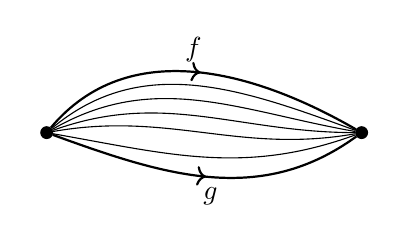
\begin{tikzpicture}
	  [decoration={markings,mark=at position 0.5 with {\arrow{>}}},
   witharrow/.style={postaction={decorate}},
   dot/.style={draw,fill,circle,inner sep=1.5pt,minimum width=0pt}
  ]


  % ellipse
  \begin{scope}[shift={(5,0)}]
    \node[dot,label={[left] }] (a3) at (5,0) {};
    \node[dot,label={[right]}] (b3) at (9,0) {};
    \draw[thick,witharrow] (a3) to[out=50,in=150]node[above]{$f$} (b3);
    \foreach \o/\i in {40/160,30/170,20/180,10/190,-10/200}
       \draw (a3) to[out=\o,in=\i]  (b3);
		\draw[thick,witharrow] (a3) to[out=-20,in=-144]node[below]{$g$} (b3);
		
  \end{scope}

\end{tikzpicture}
\caption{Picturing a homotopy between two paths $f$ and $g$.}
\end{figure}

\indent Additionally, for any two paths $f,g: [0,1] \to X$ where $f(1) = g(0)$ we can define their composition $f \circ g: [0,1] \to X$ where $(f \circ g )(t) = f(t)$ for $0 \leq t \leq \frac{1}{2}$ and $(f \circ g)(t) = g(2t - 1)$ for $ \frac{1}{2} < t \leq 1$ which we may think of as concatenating the two paths.
Of particular interest to us, any two paths starting and ending at the same point can be composed.

\begin{proposition}
	For a topological space $X$ and a choice of a basepoint $x \in X$, concatenation of loops which start and end at $x$ forms a group when restricted to homotopy classes.
\end{proposition}

This is a straightforward check. 
In particular, the identity is the homotopy class of the constant loop $s: [0,1] \to x \in X$ and the inverse of a homotopy class of the loop $s: [0,1] \to X$ is the homotopy class of the "backwards" path $s(1-t)$.
This already allows us to define the topological fundamental group.
\begin{definition}[Topological Fundamental Group]
	For a space $X$ with basepoint $x$, the (topological) \textit{fundamental group} $\pi^{\text{top}}_1(X,x)$	is the group of homotopy classes of loops with origin in $x$.
	The group operation is the same composition of loops defined previously.
\end{definition}

\begin{examples} \text{} 
	\begin{enumerate}
		\item The circle $S^1$ has fundamental group $\Z$. 
			Picking a basepoint of $S^1$ the identification $\pi_1^{\text{top}}(S^1,x)$ identifies a loop with the number of times it winds around.
			Which loops correspond to positive numbers or negative correspond to a choice of orientation of $S^1$ (an identification of clockwise or counterclockwise). 
		\item For any $n$, $\R^n$ has trivial fundamental group, such spaces are called \textit{simply connected}.
			Indeed, any loop $s: [0,1] \to \R^n$ with end $x $can be "drawn in" to $x$ by the homotopy $s_t(y) = (1-t)s(y) + tx$.
	\end{enumerate}
	
\end{examples}

As mentioned, it is not immediately clear how to generalize this definition of the fundamental group to the scheme case.
It is intead from the viewpoint of coverings that we will eventually develop it for schemes, hence we begin to establish its relation with the topological fundamental group.

\begin{definition}[Covering Spaces]
A cover of $X$ consists of a topological space $Y$ and a map $p:Y \to X$ that satisfies the following property. 
	For all $x \in X$ there exists an open neighborhood $U$ of $x$ where $p^{-1}(U)$ decomposes into a nonempty disjoint union of open subsets $V_i$ of $X$ such that each map homeomorphically onto $U$ under $p$.
\end{definition}

Under the above conditions we may also call $Y$ a \textit{covering} of $X$.
We will be interested in the case when the fibers $p^{-1}(x)$ of a cover are finite for all $x \in X$ which we will call $Y$ a \textit{finite cover} or \textit{finite covering} of $X$.
A \textit{trivial cover} of $X$ is the natural projection $X \times I \to X$ for $I$ a discrete set, which looks like multiple copies of $X$ each mapping homeomorphically onto $X$.
With this in mind, the condition in the definition of Covering Spaces may be phrased as locally trivial, in that the map when restricted to a small enough neighborhood looks like a trivial cover.
Note that some authors require a covering space to be connected, we will not follow this convention and will explicitly state whenever $Y$ is connected.


\begin{figure}[ht!]
\centering
\includegraphics[width=50mm]{CoveringSpace.png}

\caption*{A covering the figure eight space [\cite{FomenkoFuchs}, \textbf{Fig. 29}]}
\end{figure}

\begin{example} Suppose that a topological group $G$ acts discretely on a space $Y$, that is, every $y \in Y$ has an open neighborhood $V$ such that the open sets $gV$ are pairwise disjoint for all $g  \in G$.
	Then the natural projection $Y \to G/Y$ under this action is a projection.
	For example, $\Z$ acts on $\R$ discretely by translation via the map $\Z \times \R \to \R$ sending $(n,r) \to n+r$.
	The corresponding cover $\R \to \R/\Z$ is a covering of $\R/\Z$ which is homeomorphic to $S^1$.
\end{example}

\indent A map between two covers $p_1: Y_1 \to X, p_2: Y_2 \to X$ is a continuous map $f: Y_1 \to Y_2$ making the below diagram commute.
% https://q.uiver.app/#q=WzAsMyxbMCwwLCJZXzEiXSxbMiwwLCJZXzIiXSxbMSwxLCJYIl0sWzAsMiwicF8xIl0sWzEsMiwicF8yIiwyXSxbMCwxLCJmIl1d
\[\begin{tikzcd}
	{Y_1} && {Y_2} \\
	& X
	\arrow["f", from=1-1, to=1-3]
	\arrow["{p_1}", from=1-1, to=2-2]
	\arrow["{p_2}"', from=1-3, to=2-2]
\end{tikzcd}\]
From the commutativity, we see that for any $x \in X$ the map $f$ restricts to map between the fibers $p_1^{-1}(x)$ and $p_2^{-1}(x)$.\\
\indent Now these maps along with the objects consisting of covers over $X$ defines a category.
Hence for each cover $p:Y \to X$ there is a group of automorphisms consisting of the maps $f: Y \to Y$ such that $f = f \circ p$.
We will denote this group as $\text{Aut}(Y|X)$ from now on, and call its elements \textit{deck transformations} following \cite{FomenkoFuchs}.
Now deck transformations must map fibers $p$ bijectively onto each other, which leads us to consider the following types of covers.

\begin{definition}[Regular Covers]
	A connected cover $p: Y \to X$ is \textit{regular} if the group of deck transformations acts transitively on each fiber.
\end{definition}

We will not immediately make use of this definition, but it will be handy to keep in mind.
The following lemma will be necessary in relating the topological fundamental group with covers.

\begin{proposition}[Lifting Paths and Homotopies]	
	Let $p: Y \to X$ be a covering. 
	For any $\widetilde{x} \in Y$, and path $s: [0,1] \to X$ such that $s(0) = x = p(\widetilde{x})$, there exists a unique path $\widetilde{s}:[0,1] \to Y$ such that $\widetilde{s}(0) = \widetilde{x}$ and $p \circ \widetilde{s} = s$.
	In addition, if $s_1, s_2$ are two homotopic paths in $X$, their lifts $\widetilde{s_1}$ and $\widetilde{s_2}$ are homotopic in $Y$.
\end{proposition}

\begin{proof}
	The local triviality allows us to explicitly construct the lift of the path, for a full proof of the two statements see \cite{FomenkoFuchs}, Lecture 6.5.
	There you may also find stronger lifting theorems, but for our purposes this is all we need.
\end{proof}
		
Consider a covering $p: Y \to X$ and let $x \in X$ be a chosen basepoint and $y$ an element of the fiber $p^{-1}(x)$.
	For any path $s$ representing a class $[\alpha] \in \pi_1(X,x)$ there is a unique lift $\widetilde{s}$ from the previous proposition.
	Define an action of $\pi_1(X,x)$ on the set $p^{-1}(x)$ by letting $[\alpha] \circ y = \widetilde{s}(1)$.
	Since $\widetilde{s}(1)$ is the same for homotopic paths, this action is well-defined by the last part of the previous proposition.
	We will call this (left) continuous action on $p^{-1}(x)$ the \textit{monodromy action}.\\
	\indent There is then a functor $\text{Fib}_x$, which takes a cover $Y \to X$ to the finite fiber $p^{-1}(x)$ of the basepoint.
The culmination of the work in this section is to describe the following theorem.
We require some niceness conditions on the space $X$, one of which is that of \textit{locally simply connectedness}, which requires that for every $x \in X$ a neighorhood which is simply connected.

	\begin{theorem}\thlabel{coverfunctor}
	For a connected and locally simply connected space $X$ with base point $x$, the functor $\text{Fib}_x$ induces an equivalence between the category of finite covers of $X$ and the category of finite continuous left $\widehat{\pi_1(X,x)}$-sets.
	Connected covers correspond to finite $\widehat{\pi_1(X,s)}$-sets with transitive action and Galois covers correspond to space of open normal subgroups.
\end{theorem}
\begin{proof}
	The proof first shows an equivalence between $\pi_1(X,x)$ sets and arbitrary covers of $X$ by showing that the functor is in fact representable by an aptly named \textit{universal cover} $\widetilde{X} \to X$.
The profinite completion of $\pi_1(X,x)$ arises in the case of finite covers as its corresponding actions factor through some finite quotient.
	For all the details see Theorem 2.3.5 and Corollary 2.3.9 in \cite{Szamuely}.
\end{proof}


Compare with \thref{grothendiecksformulation}.
One may already conjecture the below relations
\begin{center}
\begin{tabular}{ |c c c| } 
\hline
	Absolute Galois Groups & $\Longleftrightarrow$ & $\widehat{\text{Fundamental Group}}$ \\
 
	Galois Extensions & $\Longleftrightarrow$ & Regular Coverings\\
 
	Separable Extensions & $\Longleftrightarrow$ & Connected Coverings\\
 \hline
\end{tabular}
\end{center}

One way to resolve this is with the notion of a \textit{Galois category} (see \cite{grothendieck} or \cite{Lenstra} for those interested in a detailed treatment), which both our category of finite \'etale $k$ algebras and finite covers are incarnations of. 
As one may speculate, any Galois category is equivalent to a category of finite $G$-sets for a profinite group $G$.
In our cases so far Galois extensions and regular coverings as well as separable extensions and connected coverings are respectively instances of \textit{Galois objects} and \textit{connected objects} in a Galois category.
We will not go over these treatments, but it may be useful to keep in mind the parallels especially as we begin develop another Galois category but in the context of schemes.

\todo{Give motivations}


\section{The Algebraic Fundamental Group}

We can now start defining the scheme analogue of the fundamental group.
Setting up the correct notion of a finite cover for schemes requires a lot of care which we will start to go through.

\subsection{Finite \'Etale Covers}

We being with some preliminary definitions and start to familiarize ourselves with some important properties.

\begin{definition}[Finite morphism]
	An affine morphism $f: X \to Y$ of schemes is called \textit{finite} if for some affine open cover $\{U_i\}_{i \in I}  = \{\text{Spec}(A_i)\}_{i \in I}$ where $f^{-1}(U_i) = \text{Spec}(B_i)$, the natural ring homomorphism $A_i \to B_i$ exhibits $B_i$ as a finitely generated $A_i$-module.
\end{definition}

\begin{example}
	A closed immersion is finite as closed immersions are affine and the induced maps $\text{Spec}(A) \to \text{Spec}(A/I)$ are induced by surjective ring maps.
\end{example}

The most important aspect of finite morphisms for us is as follows.
\begin{proposition}
	A finite morphism $f: X \to Y$ is proper. 
\end{proposition}
\begin{proof}
	We make use of the valuative criterion (\cite{stacks-project}, \textbf{29.42}).
	Finite morphisms are automatically of finite type, and since they are affine they are also quasi-separated.
	Hence it suffices to show that for any valuation ring $R$ with field of fractions $K$ and commutative diagram
	% https://q.uiver.app/#q=WzAsNCxbMCwxLCJcXHRleHR7U3BlY30oUikiXSxbMCwwLCJcXHRleHR7U3BlY30oSykiXSxbMSwwLCJYIl0sWzEsMSwiWSJdLFsxLDJdLFswLDNdLFsyLDNdLFsxLDBdXQ==
\[\begin{tikzcd}
	{\text{Spec}(K)} & X \\
	{\text{Spec}(R)} & Y
	\arrow[from=1-1, to=1-2]
	\arrow[from=1-1, to=2-1]
	\arrow[from=1-2, to=2-2]
	\arrow[from=2-1, to=2-2]
\end{tikzcd}\]
that there exists a unique lift $\ell: \text{Spec}(R) \to X$ commuting with the diagram.
Denote $y \in Y$ the image of the generic point of $\text{Spec}(R)$, and consider an affine open $\text{Spec}(A)$ containing $y$.
It must also contain the closure of $y$ and hence the entire image of $\text{Spec}(R)$.
And letting $\text{Spec}(B) = f^{-1}(\text{Spec}(A))$, the above says that any lift $\ell$ must factor through the inclusion of $\text{Spec}(B)$.
In addition, any lift to $\text{Spec}(B)$ that commute with its map to $\text{Spec}(A)$ defines a lift of $f$, hence we may assume that $X$ and $Y$ are affine.
Then if $X = \text{Spec}(B'), Y = \text{Spec}(A')$, it suffices to show there is a unique ring homomorphism making the following diagram commute.
% https://q.uiver.app/#q=WzAsNCxbMCwxLCJSIl0sWzAsMCwiSyJdLFsxLDEsIkEnIl0sWzEsMCwiQiciXSxbMCwxLCIiLDEseyJzdHlsZSI6eyJ0YWlsIjp7Im5hbWUiOiJob29rIiwic2lkZSI6InRvcCJ9fX1dLFsyLDAsImMiXSxbMywxLCJkIiwyXSxbMiwzLCJmJyIsMl0sWzMsMCwiXFxwaGkiLDFdXQ==
\[\begin{tikzcd}
	K & {B'} \\
	R & {A'}
	\arrow["d"', from=1-2, to=1-1]
	\arrow["\phi"{description}, from=1-2, to=2-1]
	\arrow[hook, from=2-1, to=1-1]
	\arrow["{f'}"', from=2-2, to=1-2]
	\arrow["c", from=2-2, to=2-1]
\end{tikzcd}\]
Since $f'$ exhibits $B'$ as a finitely generated $A'$-module, every element of $B'$ is integral over $A'$.
However, since $R$ is a valuation ring it is closed in its field of fractions $K$, hence the image of $B'$ under $d$ must be contained in $R$.
This precisely says that $d$ factors through the inclusion $R \hookrightarrow K$, giving us our desired unique map.
\end{proof}


For a morphism $f: X \to Y$ of schemes the map $f^{\flat}: \mc{O}_Y \to f_*\mc{O}_X$ exhibits the direct image sheaf $f_* \mc{O}_X$ as an $\mc{O}_Y$-algebra.
In particular, $f_* \mc{O}_X$ is also an $\mc{O}_Y$-module.
This allows us to make the next definition.

\begin{definition}[Locally free morphism]	
	A finite morphism $f: X \to S$ is \textit{locally free} if the direct image sheaf $f_* \mc{O}_X$ is locally free of finite rank.   
\end{definition}

We can now define our main morphism of interest.
Immediately afterward we will record some basic properties we would expect.
\begin{definition}[Finite \'etale morphism]
	A locally free morphism $f$ where for each $s \in S$, the fiber $X_s$ is a finite \'etale $\kappa(s)$-algebra is called a \textit{finite \'etale morphism}.
	If $f$ is also surjective (on space) we may call $f$ a \textit{finite \'etale cover}.
\end{definition}

There is a lot involved in the formulation of finite \'etale morphisms so we give some examples to digest.

\begin{examples}\text{} 
	\begin{enumerate}
\item 	A \textit{trivial cover} of a scheme $X$ consists of the disjoint union of copies of $\coprod_{i \in I} U$, and the natural map $p: \coprod_{i \in I} U \to U$ which when restricted to each $U$ is the identity.
	The pre-image of an affine open $\text{Spec}(A)$ of $X$ is $\coprod_{i \in I} \text{Spec}(A)$.
	When the indexing set $I$ is finite we have $\coprod_{i \in I} \text{Spec}(A) \cong \text{Spec}(A \times \dots \times A)$.
	Hence it is then readily verified that $p$ is a finite \'etale cover.
\item  Let $B = A[x]/(f)$  for some ring $A$ and monic polynomial $f \in A[x]$ of degree $d$.
	Then the natural map $\phi: \text{Spec}(B) \to \text{Spec}(A)$ is finite \'etale if $(f, f') = (1)$.
	Indeed, $\phi$ is trivially affine, and is both finite and locally free as $B$ is freely generated as an $A$-module by the elements $1,x, \dots x^{d-1}$.
	And for $\mk{p} \in \text{Spec}(A)$, the corresponding fiber is $B \otimes_A \kappa(\mk{p}) \cong \kappa(\mk{p})[x]/(\overline{f})$ for $\overline{f})$ the image of $f$ in $\kappa(\mk{p})[x]$.
	When $(f, f') = (1)$ the roots are simple, and so define a finite \'etale $\kappa(\mk{p})$-algebra hence $\phi$ is finite \'etale.
    \end{enumerate}	 
\end{examples}

\begin{remark}
	As is very often the case in algebraic geometry, there are often many equivalent formulations of some concept.
	This is indeed the case for finite \'etale morphisms as well and we will quickly give a separate definition as well which will be more useful later on.
	As one may expect, finite \'etale is equivalent to some finiteness condition and a notion of being \textit{\'etale} which we will begin to define.

\end{remark}

\begin{definition2}[Unramified morphisms]
	A morphism $f: X \to Y$ which is locally of fintie type is also said to be \textit{unramified} at $x \in X$ if $\mc{O}_{X,x}/\mk{m}_{f(x)} \mc{O}_{X,x}$ is a finite separable field extension of $\mc{O}_{X, f(x)}/\mk{m}_{f(x)}$.
\end{definition2}


\begin{definition2}[\'Etale morphisms]
	A morphism $f: X \to Y$ is called \textit{\'etale} if it is flat and unramified.
\end{definition2}

\begin{proposition}
	A morphism $f: X \to Y$ of schemes is finite \'etale if and only if it is finitely presented and \'etale.
\end{proposition}
\begin{proof}
	See 6.9 Proposition in \cite{Lenstra}
\end{proof}

\begin{remark}
	There are many potential motivations we could delve into for these choice of definitions, from local isomorphisms of manifolds to unramified extensions in algebraic number theory.
While we will briefly touch on the latter topic, we won't be able to fully touch on all of these connections.
For an interested reader however, \cite{milneLEC} provides a good discussion on flat and unramified maps. 
\end{remark}

We now record some basic (but very useful!) results one would expect of any reasonable morphism of schemes.

\begin{proposition}\thlabel{basicresults}
The following hold for finite \'etale morphisms: 
\begin{enumerate}
	\item Finite \'etale morphisms are closed under base change and composition
	\item If $f: X \to S$ is an \'etale morphism, then ths diagonal morphism $X \to X \times_S X$ induced by $f$ is an isomorphism of $f$ onto an open and closed subscheme of $X \times_S X$.
\end{enumerate}
\end{proposition}

\begin{proof}
	See \cite{Szamuely}, Proposition 5.2.7. and Proposition and Remarks 5.2.3
\end{proof}

\begin{proposition}\thlabel{cancellation}
	Let $f\colon X \to S$ and $G: Y \to X$ be morphisms of schemes. 
	Then 
	\begin{enumerate}
		\item If $f \circ g$ is finite and $f$ is separated, then $g$ is finite.
		\item If in addition both $f \circ g$ and $f$ are finite \'etale, then so is $g$.
	\end{enumerate}
	
\end{proposition}

\begin{proof}	
	For the first statement, since $f$ is separated, it diagonal $\Delta_f$ is a closed immersion, and so also finite. 
	Since finite morphisms are closed under composition and base change, the Cancellation Theorem (11.21 \cite{therisingsea}) gives us that $g$ must be finite as well.\\
\indent The second proposition follows similarly, since $f$ is finite \'etale \thref{basicresults} tells us that its diagonal $\Delta_f$ is an immersion onto on open and closed subscheme, which is also finite \'etale.
As \thref{basicresults} tells us that finite 'etale morphisms are closed under composition and basechange, the Cancellation Lemma tells us that $g$ is also finite \'etale.
\end{proof}

\begin{proposition}
	The image of a finite and locally free morphism $f: X \to Y$ (in particular a finite \'etale cover) is both open and closed.
\end{proposition}

\begin{proof}
	The image is closed because a finite morphism is proper and hence closed.
	To show that it is open, consider any point $y$ in the image of $f$, as $f_* \mc{O}_X$ is locally free as an $\mc{O}_Y$-module, there is an open neighborhood $U$ of $f$ such that 
	\[(f_* \mc{O}_X)|_U \cong (\mc{O}_Y|_U)^{\oplus n}\]
	But this says that $U$ must be contained in the image of $f$, hence its image must also be open.
\end{proof}

With all most of the technical details behind us, we can begin to construct the correct analog of fibers from the topological case.

\begin{definition}[Geometric Point]
	Let $X$ be a scheme and consider a map $\overline{x}: \text{Spec}(k) \to X$ for $k$ a field.
	Denote $x \in X$ the image of the unique point of $\text{Spec}(k)$ under $\overline{x}$.
	We say $\overline{x}$ is a \textit{geometric point} if the field extension $\kappa(x) \supset k$ is a separable closure of $k$.
\end{definition}

\begin{definition}[Geometric Fiber]
	Let $S$ be a scheme. 
	Given a morphism $f: X \to S$ and a geometric point $\overline{x}: \text{Spec}(k) \to X$ the \textit{geometric fiber} $X_{\overline{x}}$ is the fiber product $\text{Spec}(k) \times_S X$ induced by $f$ and $\overline{x}$.
\end{definition}

\begin{remark}
As a result of \thref{etalealgebra} for finite dimensional \'etale algebras over a field, the geometric fiber of a finite \'etale morphism $f: X \to S$ for a geometric point $\overline{s} : \text{Spec}(\Omega) \to S $ is isomorphic to the finite disjoint union $\text{Spec}(\Omega \times \dots \times \Omega)$ of copies of $\text{Spec}(\Omega)$, which one may view as analogous to the finite fibers in the topological case.
\end{remark}

In pursuit of this connection, one may again for a map of schemes $f: X \to S$ denote $\text{Aut}(X|S)$ as the set of automorphisms of $X$ consisting of the maps $\lambda$ such that $f  = f \circ \lambda$.
This will indeed still be the correct notion, in the case where $f$ is finite \'etale consider the following diagram
% https://q.uiver.app/#q=WzAsNixbMSwxLCJYIl0sWzAsMSwiUyJdLFswLDAsIlxcdGV4dHtTcGVjfShcXE9tZWdhKSJdLFsxLDAsIlxcdGV4dHtTcGVjfShcXE9tZWdhKVxcdGltZXNfUyBYIl0sWzIsMSwiWCJdLFsyLDAsIlxcdGV4dHtTcGVjfShcXE9tZWdhKVxcdGltZXNfUyBYIl0sWzAsMV0sWzIsMSwiXFxvdmVybGluZXtzfSJdLFszLDJdLFszLDBdLFszLDEsIiIsMSx7InN0eWxlIjp7Im5hbWUiOiJjb3JuZXIifX1dLFs0LDAsIlxcbGFtYmRhIiwxXSxbNSwzXSxbNSw0XSxbNSwwLCIiLDEseyJzdHlsZSI6eyJuYW1lIjoiY29ybmVyIn19XV0=
\[\begin{tikzcd}
	{\text{Spec}(\Omega)} & {\text{Spec}(\Omega)\times_S X} & {\text{Spec}(\Omega)\times_S X} \\
	S & X & X
	\arrow["{\overline{s}}", from=1-1, to=2-1]
	\arrow[from=1-2, to=1-1]
	\arrow["\lrcorner"{anchor=center, pos=0.125, rotate=-90}, draw=none, from=1-2, to=2-1]
	\arrow[from=1-2, to=2-2]
	\arrow[from=1-3, to=1-2]
	\arrow["\lrcorner"{anchor=center, pos=0.125, rotate=-90}, draw=none, from=1-3, to=2-2]
	\arrow[from=1-3, to=2-3]
	\arrow[from=2-2, to=2-1]
	\arrow["\lambda"{description}, from=2-3, to=2-2]
\end{tikzcd}\]
By definition the leftmost square and the entire rectangle, but by gluing of pullbacks this means the righthand square is also a pullback.
As $\lambda$ is an isomorphism, so is the induced map on the geometric fiber $\text{Spec}(\Omega)\times_S X$, hence $\text{Aut}(X|S)$ has a natural action on geometric fibers for a given geometric point.

\begin{proposition}
	Let $S$ be a connected scheme, and $f\colon X \to S$ an affine surjective morphism.
	Then $f$ is a finite \'etale cover if and only if there is a finite, locally free and surjective morphism $g: Y \to S$ such that $X \times_S Y$ is a trivial cover of $Y$.
\end{proposition}
\todo{Probably not necessary}

\begin{lemma}
	Let $X, Z$ be two $S$-schemes where $Z$ is connected and $X$ finite \'etale (over $S$). 
	If $f_1, f_2: Z \to X$ are two $S$-scheme morphisms and $\overline{z}$ a geometric point of $Z$  such that $f_1 \circ \overline{z} = f_2 \circ \overline{z}$ then $f_1 = f_2$.
\end{lemma}

\begin{proof}
	\todo{Fill in}
\end{proof}

It is an easily-proven theorem that automorphisms of covering spaces in the topological case are uniquely determined by the image of a single point; this is due to certain lifting properties (see Proposition 1, Lecture 6.8, \cite{FomenkoFuchs}).
In this spirit,we obtain as a corollary of the above that automorphisms of connected finite \'etale covers are determined uniquely by their images on geometric points.
\begin{corollary}\thlabel{finitepoints}
	If $f: X \to S$ is a connected finite \'etale cover, then nontrivial elements of $\text{Aut}(X|S)$ act without any fixed points on any geometric fiber.
	In particular, $\text{Aut}(X|S)$ is finite.
\end{corollary}

\begin{proof}
	For any nontrivial automorphism $\lambda$ of $X$, apply the previous proposition where $f_1, f_2$ are $\text{id}_x$ and $\lambda$ respectively.
\end{proof}

With the notion of an action on the fibers of a cover, we have an analogous definition to that in the topological case.

\begin{definition}[Finite \'etale Galois cover]
	A connected finite \'etale cover $X \to S$ is called \textit{Galois} if $\text{Aut}(X|S)$ acts transitively on every geometric fiber.
\end{definition}


\subsection{The \'Etale Fundamental Group}


We are now in a similar situation as when we defined the topological fundamental group.
Let $\text{Fet}_S$ denote the category of finite \'etale covers of $S$.
Fix a geometric point $\overline{s}$ of $S$, there is a natural functor to the category of finite sets \textbf{FinSet} by taking the geometric fiber over $\overline{s}$. 
The analogy of the monodromy action, on the other hand, is not immediately obvious.
We instead consider the following.

\begin{definition}[The \'Etale Fundamental Group]
	For a scheme $S$ and a geometric point $\widetilde{s}: \text{Spec}(K) \to S$, we define the \textit{\'etale fundamental group} $\pi_1(S, \widetilde{s})$ as the automorphism group of the fiber functor $\text{Fib}_{\overline{s}}$ from $\text{Fet}_{S}$ to $\textbf{FinSet}$.
\end{definition}

Here we are viewing the fiber functor as an object of the category consisting of functors from $\text{Fet}_S$ to $\textbf{Fin}$ in which case automorphisms consist of natural isomorphisms of functors.\\

We now give a vital proposition, which is an analog of the fact that every finite separable field extension is embedded into some finite Galois extension.  


\begin{proposition}\thlabel{unigal}
	Let $f: X \to S$ be a connected finite \'etale cover. 
	There is a morphism $\pi: P \to X$ such that $f \circ \pi: P \to S$ is a finite \'etale Galois cover, and moreover for every $S-$scheme morphism $\phi:K  \to X$ where $K$ is Galois factors through $\pi$.
\end{proposition}

\begin{proof}
	See \cite{Szamuely}, Proposition 5.3.9
\end{proof}

In the topological case the functor $\text{Fib}_x$ was in fact representable by the so called universal cover, and our functor in \thref{grothendiecksformulation} by the separable closure $k^s$.
However $k^s$ need not be a finite separable extension less a finite \'etale $k$-algebra so it is not representable as in the sense of the topological group.
Despite this, there is a somewhat weaker notion of representability called \textit{pro-representability} which is satisfied.


\begin{definition}[Pro-representable functors]
	Let $C$ be a category and $F: C \to \text{Set}$ a set-valued functor.
	We will say that $F$ is \textit{pro-representable} if it is the colimit of an inverse system $(P_{\alpha}, \phi_{\alpha \beta})$ in the category $\text{Set}^C$ of set valued-functors with indexing objects representable presheaves, in which case we will write 
\[F \cong \varinjlim \text{Hom}(P_{\alpha}, -)\]
\end{definition} 

Note that as opposed to an inverse limit, we are instead taking the colimit as opposed to the limit.
Since the colimit takes values in presheaves, it is in fact defined termwise.
This says that for any object $C$, restricting the functors to $C$ preserves colimits; we know what colimits look like in Set, they are the disjoint union of sets in the diagram, modulo the equivalence where two elements are identified if they are mapped to some common element in the diagram. 
With this in mind we now begin to develop some necessary background regarding the \'etale fundamental group.
Recall that $k^s$ can be thought of as the union of its finite Galois subextensions.
In fact, the functor to \textbf{FinSet} associated to each Galois category is pro-represented by its Galois objects; we outline this below for $\text{Fib}_{\overline{s}}$.

\todo{Fill in below proofs}
\begin{proposition}\thlabel{prorepresentation}
	Let $X$ be a finite \'etale $S$-scheme and $\overline{s}$ a geometric point of $S$.
	Then the fiber functor $\text{Fib}_{\overline{s}}$ is pro-representable.
\end{proposition}

\begin{proof}
	We will give a detailed outline of the proof.
	There is a partially ordered set consisting of all finite \'etale Galois covers $P_{\alpha} \to S$, and where we let $P_{\alpha} \leq P_{\beta}$ if there is a morphism of covers $P_{\beta} \to P_{\alpha}$.
	One can show it is directed by constructing a map using \thref{unigal}.\\
	\indent There is no immediate choice of maps in our inverse system.
	However, if for every $P_{\alpha}$ in our partially ordered set we fix an element $p_{\alpha}$ in the geometric fiber $\text{Fib}_{\overline{s}}(P_{\alpha})$ there are such maps.
	In particular, since the covers are Galois and automorphisms act transitively on the fibers, if $P_{\alpha} \leq P_{\beta}$ there exists a unique map $\phi_{\alpha \beta}: P_{\beta} \to P_{\alpha}$ such that $\text{Fib}_{\overline{s}}(\phi_{\alpha \beta})(p_{\beta}) = p_{\alpha}$, so the maps respect the chosen geometric points.
	Then for any finite \'etale cover $P_{\alpha}$, there exists by Yoneda Lemma a unique natural transformation $\text{Hom}(P_{\alpha}, -)$ to $\text{Fib}_{\overline{s}}$ sending $\text{id}_{P_{\alpha}} \in \text{Hom}(P_{\alpha}, P_{\alpha})$ to $p_{\alpha} \in \text{Fib}_{\overline{s}}(P_{\alpha})$.
	By the uniqueness of these natural transformations, they must commute with the natural transformations $\text{Hom}(P_{\alpha}, -) \to \text{Hom}(P_{\beta}, -)$ given by pre-composing with $\phi_{\alpha \beta}$, and hence in total define a natural transformation from the colimit
	\[\varinjlim \text{Hom}(P_{\alpha}, -) \to \text{Fib}_{\overline{s}}\]
	To define the inverse natural transformation, for any finite \'etale cover $X \to S$ and $x \in \text{Fib}_{\overline{s}}(X)$ we consider the promised finite \'etale Galois cover $P$ from \thref{unigal}.
	Since $P$ is Galois it is some $P_{\delta}$ in our inverse system and so in addition there exists a unique map $\varphi: P_{\delta} \to X$ mapping $p_{\delta}$ to $x$.
The inverse map sends $x$ back to the representative of $\varphi$ in $\varinjlim \text{Hom}(P_{\alpha}, X)$.

\end{proof}

Notice that in the above proof, in order to specify the maps defining the inverse system of any pro-representation we had to choose geometric points for each object in our system, but is unique afterwards.
In fact, note that a natural isomorphism of $\text{Fib}_{\overline{s}}$ under the its pro-representation above must map the system of elements $p_{\alpha}$ to another system of elements $p'_{\alpha}$ consisting automorphisms for each $P_{\alpha}$.
As each $P_{\alpha}$ is Galois over $S$, there is a unique $ \lambda \in \text{Aut}(P_{\alpha}|S)$ such that $\text{Fib}_{\overline{s}}(\lambda)(p_a) = p'_a$.
By uniqueness these then also form an inverse system and so define a pro-representation of $\text{Fib}_{\overline{s}}$ giving us the following corollary.

\begin{corollary}
	Every automorphism of the functor $\text{Fib}_{\overline{s}}$ comes from a unique automorphism of the inverse system constructed in the above proof.
\end{corollary}

With this in hand, we can finally get our hands on a somewhat more concrete description of the \'etale fundamental group.

\begin{corollary}
	The automorphism groups $\text{Aut}(P_{\alpha})^{\text{op}}$ form an inverse system whose limit is isomorphic to $\pi_1(S, \overline{s})$.
\end{corollary}

\begin{proof}
	
	If $\alpha \leq \beta$, consider the corresponding map $\phi_{\alpha \beta}: P_{\beta} \to P_{\alpha}$; it is also finite \'etale by \thref{cancellation}.
	Any automorphism $\lambda \in \text{Aut}(P_{\beta}|S)$ determines some unique element in $\text{Fib}_{\overline{s}}(P_{\beta})$ as $P$ is Galois, and hence an unique element in $\text{Fib}_{\overline{s}}(P_{\alpha})$ from the natural map induced by $\phi_{\alpha \beta}$.
By the same argument this corresponds to a unique element in $\text{Aut}(P_{\alpha}|S)$, as this respects composition of automorphisms there is thus a natural group homomorphism $\text{Aut}(P_{\alpha}|S) \to \text{Aut}(P_{\beta}|S)$.
Now from the previous corollary, automorphisms of the fiber functor correspond to systems of elements in the fiber.
But these are precisely elements in the profinite group $\varprojlim P_{\alpha}$ from its explicit description.
Since our pro-representation was represented by $\text{Hom}(P_{\alpha}, -)$, the actions of the automorphism are naturally viewed from the right, hence the opposite on the acting groups.
\end{proof}

\begin{theorem}[Grothendieck]\thlabel{etalefunctor}
	Let $S$ be a connected scheme, and $\overline{s}: \text{Spec}(K) \to S$ a geometric point. Then \begin{enumerate} 
		\item The group $\pi_1(S, \overline{s})$ is profinite, and its action on $\text{Fib}_{\overline{s}}(X)$ is continuous for all $X$.
		\item The functor $\text{Fib}_{\overline{s}}$ induces an equivalence between $\text{Fet}_S$ and the category of finite continuous (left) $\pi_1(S, \overline{s})$-sets.	In addition, connected covers correspond to sets with transitive action, and Galois covers to finite quotients of $\pi_1(S, \overline{s})$.
 \end{enumerate} 
\end{theorem}

\begin{proof}
	There is a pro-representation by a system $(P_{\alpha}, \phi_{\alpha \beta})$  by \thref{prorepresentation}.
	As we showed that automorphism groups are finite from \thref{finitepoints}, the previous corollary gives us that $\pi_1(S, \overline{s})$ is profinite from definition.
To show that the action is continuous, note that  
\end{proof}

\begin{remark}
As a corollary we now give the promised proof of \thref{grothendiecksformulation}.
Let $S = \text{Spec}(k)$ for $k$ a field; a finite \'etale cover corresponds to the affine scheme of a finite dimensional \;etale $k$-algebra $L$.
For a geometric point $\text{Spec}(\Omega) \to S$, the corresponding geometric fiber is the pullback of affine schemes $\text{Spec}(\Omega \otimes_k L)$, which as a set it is indexed by all $k$-algebra homomorphisms from $L$ to $\Omega$ \todo{Elaborate with primitive element theorem}.
Since the image of every map must lie in the separable closure of $k$ within $\Omega$, we have an isomorphism 
\[\text{Fib}_{\overline{s}}(\text{Spec}(L)) \cong \text{Hom}_k(L, k^s)\]
and so we must have $\pi_1(S, \overline{s}) \cong \text{Gal}(k^s|k)$.
\end{remark}

	The topological fundamental group is functorial in that base-point preserving maps of topological spaces induce corresponding maps of their fundmantal groups, the same is in fact true in the \'etale case.
If $S, S'$ are connected schemes with $\overline{s}, \overline{s'}$ respective geometric points, a morphism $\phi: S' \to S$ such that $\phi \circ \overline{s'} = \overline{s}$ induces a functor
\[\text{BC}: \text{Fet}_S \to \text{Get}_{\overline{S}}\]
sending a cover $X$ to its basechange $X \times_S S'$, as well as morphisms $X \to Y$ to the natural morphisms $X \times_S S' \to Y \times_S S'$.
Since $\phi \circ \overline{s'} = \overline{s}$, we have $\text{Fib}_{\overline{s}} = \text{BC} \circ \text{Fib}_{\overline{s'}}$, in which case every automorphism of $\text{Fib}_{\overline{s'}}$ induces an automorphism of $\text{Fib}_{\overline{s}}$ by pre-composition with BC.
This gives us our natural map $\pi_1(S', \overline{s'}) \to \pi_1(S, \overline{s})$ induced by $\phi$.\\


In the topological case, two different choices of a basepoint for the underlying space $X$ only affected its topological fundamental group up to some inner automorphism: in particular they are still isomorphic.


We shall show what one may have to go through to calculate $\pi_1(\text{Spec}(\Z), x_0)$.
We it will require some number theoretic notions and tools, which we shall outlines as needed.

\begin{definition}
	A \textit{number field} is a finite extension of $\Q$.
\end{definition}

\begin{definition}
	If $K$ is a number field, its corresponding \textit{number ring} is the integral closure (normalization) \todo{same thing?} of $\Z \subset K$.
\end{definition}

It turns out that all number rings are examples of \textit{Dedekind domains}, which are \todo{Dedekind}
We will first make use of \textbf{Proposition 5.4.9} from \cite{Szamuely}

\begin{proposition}
	Let $S$ be an integral normal scheme.
	Denote by $K_s$ a fixed separable closure of the function field $K$ of $S$, and by $K_S$ the composite of all finite subextensions $L|K$ of $K_s$ such that the normalization of $S$ in $L$ is \'etale over $S$.
	Then $K_S|K$ is a Galois extension, and $\text{Gal}(K_S|K)$ is canonically isomorphic to the fundamental group $\pi_1(S, \overline{s})$ for the geometric point $\overline{s}: \text{Spec}(\overline{K} ) \to S$ where $\overline{K}$ is the algebraic closure of $K$ containing $K_s$.

\end{proposition}

Let us apply the above theorem to $\text{Spec}(\Z)$.
It is integral and normal as $\Z$ is a domain which is integrally closed in its field of fractions (\todo{cite}). 
Then we simply need to find all finite subextensions $L$ of its fraction field $\Q$ which is \'etale over $\Z$.
However, $L$ is by definition a number field, and the normalization of $Z$ its corresponding number ring, so we are looking for finite \'etale maps $\text{Spec}(\mc{O}_L) \to \text{Spec}(Z)$ given by the unique map $\Z \to \mc{O}_L$.



\section{The Riemann Existence Theorem}

As promised in the introduction, we will introduce the Riemann Existence Theorem and begin to explore some of its uses and consequences.
In order to transition from the \'etale context to the topological context, we will need a "nice enough" associated space to some scheme.\\

\indent If $X$ is a finite type scheme over $\C$ then for an affine open $U$ of $X$, $\Gamma(\mc{O}_X, U)$ is a finite type $\C$-algebra and so can be expressed of the form $\C[x_1, \dots, x_n]/(f_1, \dots, f_n)$ for polynomials $f_1, \dots, f_n$.
It follows $U$ is of the form $\text{Spec}(\C[x_1, \dots, x_n]/(f_1, \dots, f_n))$, of which the closed points correspond to the common zeros of $f_1, \dots, f_n$ in $\C^n$, which when viewed a subspace allows us to equip it with a natural analytic topology.
In the same way a cover of affine opens glue together to form $X$, so do their associated subspaces, giving us an associated analytic subspace $X^{\text{an}}$.
And as a map $X \to Y$ finite type schemes over $\C$ preserve closed points (the set of which is in fact a representable functor, \todo{cite}), it induces a corresponding map $X^{\text{an}} \to Y^{\text{an}}$.
This already allows us to state the Riemann Existence Theorem.


\begin{theorem}[Riemann Existence]\thlabel{RiemannExistence}\thlabel{riemannexistence}
	Let $X$ be a connected scheme of finite type over $\C$.
	Then the functor $(Y \to X) \mapsto (Y^{\text{an}} \to X^{\text{an}}))$ induces an equivalence between the categories of finite \'etale covers of $X$ and finite topological covers of $X^{\text{an}}$.
	As a result, for every $\C$ point $\overline{x}: \text{Spec}(\C) \to X$ this functor induces an isomorphism
	\[\widehat{\pi_1^{\text{top}}(X^{\text{an}}, \overline{x})} \xrightarrow{\sim} \pi_1(X, \overline{x})\]
\end{theorem}

\begin{proof}
	We will not go over the proof of the first statement, the more difficult part is in the essential surjectivity of the functor, this is overcome in $\cite{grothendieck}$ with the help of tools such as resolution of singularities.
	The relation between the two fundamental groups is an immediate application of \thref{coverfunctor}, \thref{etalefunctor}.
\end{proof}

Just working from the definition of the \'etale fundamental group, it is very difficult to figure out how to even begin computing such groups, even for simple schemes. 
As we saw at the end of the previous section that even for simple maps of field valued points given by field extensions, it is equivalent to computing their corresponding Galois groups!
However, \thref{riemannexistence} now introduces the ability to immediately begin computing certain \'etale fundamental groups using their topological analogue as we will highlight.

\begin{examples} \thlabel{Examples}\text{}
	\begin{enumerate} 	\item Consider $\textbf{A}_{\C}^1 - \{0\} \cong \text{Spec}(\C[x^{\pm 1}])$. 
		It's associated analytic space is simply $\C - \{0\}$, which has fundamental group $\Z$ for any choice of basepoint, so for any geometric point $\overline{x}$ of $\textbf{A}_{\C}^1 - \{0\}$ we conclude
		\[\pi_1(\textbf{A}_{\C}^1 - \{0\}, \overline{x}) \cong \widehat{\Z}\]
		This generalizes easily for $\textbf{A}_{\C}^n$  and localizations across more than one maximal ideal. 
		\item For $\textbf{P}_{\C}^n$, we have that its associated analytic space is just the topological complex projective space $\C P^n$.
	One may see this from the former description as gluing copies of $\textbf{A}_{\C}^n$ and the analogous set of charts on $\C P^n$.
	The topological theory gives us that 
	\[\pi_1^{\text{top}}(\C P^n, x) = 0\]
	so we conclude the same for $\pi_1(\textbf{P}_{\C}^n, \overline{x})$.
\item Topologically, complex surfaces of genus $g$ are homeomorphic to a sphere with $g$ "handles" attached.
	Using accessible tools such as a CW decomposition of the space, we can calculate the fundamental group as (see \cite{FomenkoFuchs} Lecture 7.6)
	\[\langle a_1, b_1, \dots, a_g, b_g \,|\, [a_1,b_1], \dots, [a_g,b_g] = 1\rangle \]
	with $2g$ generators, and the only relations that the commutators $[a_i, b_i] = a_i b_i a_i^{-1} b_i^{-1}$ is trivial.
\end{enumerate}
\end{examples}
\todo{picture?}
And while we have only give examples for schemes over $\C$, the below result allows us to extend it to a slightly larger class of schemes. 
\begin{proposition}
	Let $K \supset k$ be an extension of algebraically closed fields, and let $X$ be a proper integral scheme over $k$.
	Then the natural map $\pi_1(X_L, \overline{x}_K) \to \pi_1(X, \overline{x})$ is an isomorphism for all geometric points $\overline{x}$ of $X$.
\end{proposition} 

\begin{proof}
	See \cite{Szamuely}, Proposition 5.6.7.
\end{proof}

\begin{remark}
	As a general application if results about the \'etale fundamental group holds for schemes over $\C$ they hold over any field  $k$ of characteristic zero.
	To do this one would apply the above proposition for the field extensions $\overline{\Q} \hookrightarrow \C$ and then $\overline{\Q} \hookrightarrow k$ to obtain the desired isomorphism.
	For example, our previous examples for $\textbf{P}_{\C}^n$ hold whenever $\C$ is replaced with $k$ as projective space is proper and integral over a base field.
\end{remark}

\subsection{Positive Characteristic}

So far we have only made progress in the case of characteristic zero.
Certain groups, such as those interested in number theory, may wish to see if we can extend such results
to the positive characteristic case.
Thankfully results are certainly possible, albeit more difficult to formulate.
We will outline one due to Grothendieck, which for certain schemes over a field of characteristic $p \geq 0$ gives us information on the "non-$p$" part of the \'etale fundamental group by relating it to the characteristic 0 case, where one may use results such as the ones previously outlined.\\

\indent Following the notation in \cite{Szamuely} let $S$ be the affine scheme $\text{Spec}(A)$, with $\eta \colon \text{Spec}(K) \to S$ and $s \colon: \text{Spec}(\kappa) \to S$ be the generic and closed points of $S$ respectively.
Also fix geometric points $\overline{\eta}$ and $\overline{s}$ of the respective points.

\begin{theorem}[Grothendieck]
	Let $S$ be as above, and let $f: X \to S$ be a proper morphism.
	Fix geometric points $\overline{x}$ and $\overline{y}$ of $X_{\overline{\eta}}$ and $X_s$ respectively.
	\begin{enumerate}
		\item The natural map $\pi_1(X_s, \overline{y}) \to \pi_1(X, \overline{y})$ induced by the map $X_2 \to X$ is an isomorphism.
		\item Assume moreover that $k$ is algebraically closed, $\phi$ is flat, and the geometric fibers $X_{\overline{\eta}}, X_{\overline{s}}$  are reduced.
			Then the natural map $\pi_1(X_{\overline{\eta}}, \overline{x}) \to \pi_1(X, \overline{x})$
	\end{enumerate}
	
\end{theorem}

 \begin{proof}
	 Hard, \todo{cite} reference
 \end{proof}

 With the same notation as above there exists a \textit{specialization map} associated to the morphism $\phi$.
 Still assuming that $k$ is algebraically closed and that $s = \overline{s}$, then there is a composite map
 \[\textit{sp}: \pi_1(X_{\overline{\eta}}, \overline{x}) \to \pi_1(X, \overline{x}) \xrightarrow{\sim} \pi_1(X, \overline{y}) \xrightarrow{\sim} \pi_1(X_{\overline{s}}, \overline{y})\]

 The first map is from part (2) of the above theorem, the middle isomorphism coming from \todo{Paths}, and the last one is the inverse of the isomorphisms from part (1) of the theorem above.
Although there is a involved for the middle isomorphism, the resulting is still unique up to an inner automorphism.
This gives us a map relating the two fibers above a discrete valuation ring, its main use is in the below proof.

\begin{theorem}[Grothendieck] \thlabel{groth}
	Keep the same notations and assumptions as above.
	Assume that $f$ is proper and smooth with geometrically connected fibers.
	Then the specialization map induces an isomorphism 
	\[\pi_1(X_{\overline{\eta}}, \overline{x})^{p'} \xrightarrow{\sim} \pi_1(X_{\overline{s}}, \overline{y})^{p'}\]
	where the superscripts $(p')$ denote the maximal prime-to-$p$ quotients of the profinite groups involved.
	
\end{theorem}

 \begin{proof}
	 Here the maximal prime-to-$p$ quotient refers to \todo{definition}
	 Also long and involved \todo{Try and give a proof?}
 \end{proof}
 
 The main result due to Grothendieck is as follows.
\begin{theorem}
	Let $k$ be an algebraically closed field of characterstic $p \geq 0$, and let $X$ be an integral proper normal curve of genus $g$ over $k$.
	For every geometric point $\overline{x}$ of $X$, the group $\pi_1(X, \overline{x})$ has its maximal prime to $p$-quotient $\pi_1(X, \overline{x})^{(p')}$ is isomorphic to the profinite $p'$-compleiton of the group
	\[G = \langle a_1, b_1, \dots, a_g, b_g \,|\, [a_1,b_1], \dots, [a_g, b_g] = 1\rangle\]
	where $[a_i, b_i]$ denotes the commutator $a_i b_i a_i^{-1} b_i^{-1}$.
\end{theorem}

\begin{proof} We give an outline of how to proceeed.
	\begin{enumerate}
		\item We first construct a discrete valuation ring $A$ whose fraction field $K$ has characteristic 0 and whose residue field is isomorphic to $k$.
	One way is found in \todo{cite}, and we may also assume that it is complete, otherwise we may just take the completion. 
\item We then find a smooth proper scheme $Y \to \text{Spec}(A)$ such that $Y_{s} = X$ and $Y_{\eta}$ a smooth proper curve over $K$.
	There are several ways to go about this \todo{finish later}
\item Finally, we may apply \thref{groth}, as well as \thref{Examples} which gives us our desired result. 
	\end{enumerate}
	
\end{proof}

Just as above, one often finds that in the characteristic $p$ case that the "non-$p$" part is the same as in the charateristic zero.
We give the reader a taste of more results in this area (a good exposition can be found in  \cite{abhyankar}), but whose explanations are out of scope of this paper.
For a group $G$, let $p(G)$ denote the subgroup generating by all $p$-subgroups (subgroups of order a power of $p$).
One major result in this area is as follows.

\begin{conjecture}[Abhyankar's Conjecture]
	Let $X$ be a smooth projective curve of genus $g$ defined over an algebraically closed field $k$ of characteristic $p > 0$.
	Let $B$ be a non-empty set of points of $X$ having cardinality $r$ and let $U = X - B$.
	Then a finite group $G$ is a Galois group of an unramified cover of $U$ if and only if $G/p(G)$ has a generating set of size at most $2g + r -1$.
\end{conjecture}

This conjecture is in fact now a theorem, whose proof was given by Raynaud, involving the work of Serre and Harbater.
Note that in the case when $X$ is $\textbf{P}_k^1$ and $B$ is the point of infinity, then $U$ is the affine line over $k$.
Since $g = 0, r = 1$ in this case, the above theorem tells us that the Galois groups of unramified covers are precisely the \textit{quasi-p groups}, those groups which are generated by its $p$-subgroups.






\newpage
\bibliographystyle{plain}
\bibliography{lib}
\end{document}
